% Set page size and margins
\usepackage[
  a4paper,
  top=2cm,
  bottom=3cm,
  left=2cm,
  right=2cm,
  marginparwidth=1.75cm,
  footskip=2.05cm,
]{geometry}

% Useful packages
\usepackage[export]{adjustbox}
\usepackage{amsmath}
\usepackage{array}
\usepackage{caption}
\usepackage[strict]{changepage}
\usepackage{enumitem}
\usepackage{etoolbox}
\usepackage{float}
\usepackage{fullwidth}
\usepackage{graphicx, trimclip}
\usepackage[colorlinks=true, allcolors=blue]{hyperref}
\usepackage{hyperref}
\usepackage[noautomatic, nonewpage]{imakeidx}
\usepackage{multicol}
\usepackage[super]{nth}
\usepackage{outlines}
\usepackage{paracol}
\usepackage[section]{placeins}
\usepackage{setspace}
\usepackage{stfloats}
\usepackage{subcaption}
\usepackage[usetransparent=false]{svg}
\usepackage{tabularx}
\usepackage[subfigure]{tocloft}
\usepackage{tikz}
\usepackage{titlesec}
\usepackage{transparent}
\usepackage{verbatim}
\usepackage{varwidth}
\usepackage{wrapfig}
\usepackage[most]{tcolorbox}
\usepackage{catchfile}
\usepackage{xstring}
\usepackage{soul}
\usepackage{xifthen}
\usepackage{xparse}

\usepackage{tocloft}
\renewcommand{\cftsubsecpagefont}{\bfseries}

\usepackage[hang, symbol, perpage]{footmisc}
\renewcommand{\footnotemargin}{1em}

\newtcolorbox{scaledfigure}[1][]{height fill, space to=\myspace,#1}
\hypersetup{
  colorlinks=true,
  linkcolor=goldenbrown,
  filecolor=magenta,
  urlcolor=cyan,
  pdftitle={Heroes of Might \& Magic III Rule Book},
  pdfpagemode=UseNone,
}
% Set the default spacing between paragraphs. Remove indentation.
\usepackage[skip=6pt, indent=0pt]{parskip}
\setstretch{1}

% Get version from env
% \getenv{variable_name} just prints the value
% \getenv[\macro]{variable_name} stores the value in \macro for reusability
\newcommand{\getenv}[2][]{%
  \CatchFileEdef{\value}{"|echo \$#2"}{\endlinechar=-1}%
  \if\relax\detokenize{#1}\relax\value\else\let#1\value\fi}

% Add dots to the table of contents
\renewcommand{\cftsecleader}{\cftdotfill{\cftsecdotsep}}
\renewcommand\cftsecdotsep{\cftdot}
\renewcommand\cftsubsecdotsep{\cftdot}



\captionsetup[figure]{labelformat=empty}
\captionsetup[subfigure]{labelformat=empty, singlelinecheck=off, justification=centering}
\usetikzlibrary{shadows, shadows.blur, calc, backgrounds}

\setlength{\columnsep}{1cm}
\newtoggle{printable}
\newtoggle{noartbackground}
\newtoggle{githubbuild}

% Control addition of certain pages in the printable version.
% Useful to make the printable version have correct number of pages.
\newtoggle{printable_quote_separate_page}
\newtoggle{printable_notes_page}
\togglefalse{printable_quote_separate_page}
\toggletrue{printable_notes_page}

\AtBeginDocument{
  \iftoggle{printable}{}{
    % If printable was disabled, automatically disable related flags.
    \togglefalse{printable_quote_separate_page}
    \togglefalse{printable_notes_page}
  }
}

% Variables
\def\_assets{assets}

\def\art{\_assets/art}
\def\cards{\_assets/cards}
\def\examples{\_assets/examples}
\def\images{\_assets/images}
\def\layout{\_assets/layout}
\def\map_locations{\_assets/map-locations}
\def\skills{\_assets/skills}
\def\spells{\_assets/spells}
\def\svgs{\_assets/glyphs}
\def\notes_svgs{\svgs/for-notes}
\def\tables{\_assets/tables}
\def\qr{\_assets/qr-codes}

\def\repourl{https://github.com/piotrbruzda/Homm3BG-FactoryRulebook}
\def\originalrepourl{https://github.com/Heegu-sama/Homm3BG}
\def\bggthreadurl{https://boardgamegeek.com/}
% TODO: Update links

\renewcommand{\labelitemi}{\includegraphics[width=0.7em, valign=c]{\layout/listdot.png}}

% Colors
\definecolor{amber}{rgb}{1.0, 0.49, 0.0}
\definecolor{antiquewhite}{rgb}{0.98, 0.92, 0.84}
\definecolor{arylideyellow}{rgb}{0.96, 0.89, 0.58}
\definecolor{cadmiumgreen}{rgb}{0.0, 0.42, 0.24}
\definecolor{darkcandyapplered}{rgb}{0.64, 0.0, 0.0}
\definecolor{goldenbrown}{rgb}{0.6, 0.4, 0.08}

\newcommand{\svg}[2][10]{%
  {\raisebox{-0.15\height}{\includesvg[height=#1px]{\svgs/\detokenize{#2}.svg}}}%
}%
\newcommand{\svgunit}[2][10]{%
  {\raisebox{-0.1\height}{\includesvg[height=#1px]{\svgs/\detokenize{#2}.svg}}}%
}%
\newcommand{\svgeven}[2][10]{%
  \includesvg[height=#1px]{\svgs/\detokenize{#2}.svg}%
}%

% Command to insert a subsection separator image
\newcommand{\subsdivider}{%
    \begin{center}
        
\includegraphics[width=\linewidth,height=1.2em,keepaspectratio]{\layout/subsection_separator.png}
    \end{center}
    \vspace{-0.5em} % Adjust vertical spacing if needed
}

\newcommand{\subheader}[1]{%
    \begin{center}
        \textbf{\Large\scshape #1} % Wyświetlenie nagłówka bez powielenia
        \\[0.05em] % Odstęp
        
\includegraphics[width=\linewidth,height=1em,keepaspectratio]{\layout/subsection_separator.png}
    \end{center}
}




% Command to frame images
\newcommand\framedimage[2][]{%
  \begin{tikzpicture}
    \draw (0, 0) node[inner sep=0] {\makebox[#1][c]{\includegraphics[width=#1]{#2}}};
    \draw [bordermidyellow, thick] ([xshift=+1pt, yshift=-1pt] current bounding box.north west) rectangle ([xshift=-1pt, yshift=1pt] current bounding box.south east);
    \draw [borderoutyellow, thick] (current bounding box.north west) rectangle (current bounding box.south east);
    \draw [borderinyellow, thick] ([xshift=+3pt, yshift=-3pt] current bounding box.north west) rectangle ([xshift=-3pt, yshift=3pt] current bounding box.south east);
  \end{tikzpicture}}
% End of drop frame definition

\titleformat{\section}
{\huge}
{\filright
\footnotesize
\enspace SECTION \thesection\enspace}
{8pt}
{\Huge\bfseries\filcenter\uppercase}

%Create section heading with graphics. Argument one is heading name, argument two is picture to use on the left.
\providecommand{\sectionheadertext}[1]{
  \fontfamily{ptm}\selectfont{
    \color{antiquewhite} \section*{\MakeUppercase{#1}}
  }
}

\newcommand{\sectioncampaignheadertext}[2][antiquewhite]{
  \color{#1}\MakeUppercase{\textbf{\liberation #2}}
}


\newcommand{\addsection}[3][1]{
  \def\oneliner{\equal{#1}{1}}
  \vspace*{-5em}
  \hspace*{-1em}
  \makebox[0pt][l]{
  \raisebox{-\totalheight}[0pt][7pt]{
    \begin{tikzpicture}
      \draw (0, 0) node[inner sep=0] {
\includegraphics[width=\linewidth, height=0.2\linewidth]{\layout/section_heading.jpg}};
      \draw (-6.2, 0) node {\includegraphics[width=0.125\textwidth]{#3}};
    \end{tikzpicture}
    }
  }
  \begin{fullwidth}[leftmargin=0.16\textwidth, outermargin=0.16\textwidth, innermargin=0.16\textwidth]
    \begin{center}
      \vspace*{\lang_header_adjustment}
      \ifthenelse{\oneliner}{}{\vspace{-13pt}}
      \sectionheadertext{#2}
      \cleardoublepage\phantomsection\addcontentsline{toc}{section}{\protect\numberline{}\mbox{#2}}
    \end{center}
  \end{fullwidth}
  \vspace{1.75em}
  \ifthenelse{\oneliner}{}{\vspace{-13pt}}
}
%End of create section heading.

% Apply language-specific subsection spacings if defined
\ifdefined\subsectionspacing
  \subsectionspacing{}
\fi

\newcommand\picdims[4][]{%
  \setbox0=\hbox{\includegraphics[#1]{#4}}%
  \clipbox{.5\dimexpr\wd0-#2\relax{} %
    .5\dimexpr\ht0-#3\relax{} %
    .5\dimexpr\wd0-#2\relax{} %
    .5\dimexpr\ht0-#3\relax}{\includegraphics[#1]{#4}}}

\tikzset{
  thick/.style=      {line width=1.3pt},
  very thick/.style= {line width=1.7pt},
  ultra thick/.style={line width=2.2pt}
}

\definecolor{borderoutyellow}{HTML}{DBCA86}
\definecolor{borderinyellow}{HTML}{B09E69}
\definecolor{bordermidyellow}{HTML}{6f6749}
% Create note box
\providecommand{\notefont}[0]{\fontfamily{ptm}\selectfont}
\newcommand{\note}[2]{
  \begin{tikzpicture}
    \textlang{english}{\draw (0, 0) node[inner sep=0] {\makebox[\linewidth][c]{\picdims[width=\linewidth]{\linewidth}{#1\baselineskip}{\layout/table-background.jpg}}};}
    \draw [borderoutyellow, very thick] (current bounding box.north west) rectangle (current bounding box.south east);
    \draw [borderinyellow, thick] ([xshift=+2.8pt, yshift=-2.8pt] current bounding box.north west) rectangle ([xshift=-2.8pt, yshift=2.8pt] current bounding box.south east);
    \node at (current bounding box.center) {
      \begin{varwidth}{0.85\linewidth}
      \notefont{
        \color{arylideyellow}
        \hypersetup{linkcolor=amber}
        #2
        \hypersetup{linkcolor=goldenbrown}
      }
      \end{varwidth}
    };
    \begin{pgfonlayer}{background}
      \begin{scope}[blend mode=multiply]
        \draw [shade, blur shadow={shadow opacity=15}] (current bounding box.north west) rectangle (current bounding box.south east);
      \end{scope}
    \end{pgfonlayer}
  \end{tikzpicture}
}

% Four mandatory params
% - [optional] set to "subsection" or any other Level if you want to have this as a subsection in TOC
% - Lines of Campaign Name (1-2 according to the name length)
% - Campaign Name
% - Scenario Name
% - Icon
%
% TODO: possibly replace the whole \addsection with this
\newcommand{\addscenariosection}[5][section]{
  \sodef\sotitle{}{0.2em}{0.6em}{1.2em}
  \def\oneliner{\equal{#2}{1}}

  \vspace*{-5.72em}
  \hspace*{-1.3em}
  \makebox[0pt][l]{
  \raisebox{-\totalheight}[0pt][7pt]{
    \ifthenelse{\oneliner}{\def\yscale{1}}{\def\yscale{1.3}}
      \begin{tikzpicture}
        \draw (0, 0) node[inner sep=0, yscale=\yscale] (header){\makebox[1.015\textwidth][c]{
\includegraphics[width=1.055\linewidth, height=0.24\linewidth]{\layout/section_heading.png}}};
        \draw (-6.7, 0) node {\includegraphics[width=0.135\textwidth]{#5}};
      \end{tikzpicture}
    }
  }
  \begin{fullwidth}[leftmargin=0.21\textwidth]
    \begin{center}
      \vspace{\lang_header_adjustment}
      \vspace{-12pt}
      \section*{\sectioncampaignheadertext{\small{\sotitle{#3}}}}
      \vspace{\lang_header_adjustment}
      \vspace{-10pt}
      \section*{\sectioncampaignheadertext{#4}}
      \ifthenelse{\oneliner}{}{\vspace{14pt}}
      \cleardoublepage\phantomsection\addcontentsline{toc}{#1}{\protect\numberline{} {} {} {} {}#4}
      \pagetarget{#4}{}
    \end{center}
  \end{fullwidth}
  \ifthenelse{\oneliner}{\vspace{1.75em}}{\vspace{0.75em}}
  \vspace{\lang_header_adjustment}
}

% Apply language-specific subsection spacings if defined
\ifdefined\subsectionspacing
  \subsectionspacing{}
\fi

\newcommand\picdims[4][]{%
  \setbox0=\hbox{\includegraphics[#1]{#4}}%
  \clipbox{.5\dimexpr\wd0-#2\relax{} %
    .5\dimexpr\ht0-#3\relax{} %
    .5\dimexpr\wd0-#2\relax{} %
    .5\dimexpr\ht0-#3\relax}{\includegraphics[#1]{#4}}}

\tikzset{
  thick/.style=      {line width=1.3pt},
  very thick/.style= {line width=1.7pt},
  ultra thick/.style={line width=2.2pt}
}

\definecolor{borderoutyellow}{HTML}{DBCA86}
\definecolor{borderinyellow}{HTML}{B09E69}
\definecolor{bordermidyellow}{HTML}{6f6749}
% Create note box
\newcommand{\notefont}[0]{\liberation\selectfont}
\newcommand{\note}[2]{
  \begin{tikzpicture}
    \draw (0, 0) node[inner sep=0] {\makebox[\linewidth][c]{\picdims[width=\linewidth]{\linewidth}{#1\baselineskip}{\layout/table-background.jpg}}};
    \draw [borderoutyellow, very thick] (current bounding box.north west) rectangle (current bounding box.south east);
    \draw [borderinyellow, thick] ([xshift=+2.8pt, yshift=-2.8pt] current bounding box.north west) rectangle ([xshift=-2.8pt, yshift=2.8pt] current bounding box.south east);
    \node at (current bounding box.center) {
      \begin{varwidth}{0.85\linewidth}
      \notefont{
        \color{arylideyellow}
        \hypersetup{linkcolor=amber}
        #2
        \hypersetup{linkcolor=goldenbrown}
      }
      \end{varwidth}
    };
    \begin{pgfonlayer}{background}
      \begin{scope}[blend mode=multiply]
        \draw [shade, blur shadow={shadow opacity=15}] (current bounding box.north west) rectangle (current bounding box.south east);
      \end{scope}
    \end{pgfonlayer}
  \end{tikzpicture}
}







% Create Heroes-styled framed canvas for a table. Accepts three arguments:
% 1) [Optional] Drop shadow description. Use [] as the first arg to delete it.
% 2) Height specified in verses (lines of text)
% 3) Table contents like title and tabularx environment
\newcommand{\hommtable}[3][shade, blur shadow={shadow opacity=15}]{
  \begin{tikzpicture}
    \textlang{english}{\draw (0, 0) node[inner sep=0] {\makebox[\linewidth][c]{\picdims[width=\linewidth]{\linewidth}{#2\baselineskip}{\layout/table-background.jpg}}};}
    \draw [bordermidyellow, thick] ([xshift=+1pt, yshift=-1pt] current bounding box.north west) rectangle ([xshift=-1pt, yshift=1pt] current bounding box.south east);
    \draw [borderoutyellow, thick] (current bounding box.north west) rectangle (current bounding box.south east);
    \draw [borderinyellow, thick] ([xshift=+3pt, yshift=-3pt] current bounding box.north west) rectangle ([xshift=-3pt, yshift=3pt] current bounding box.south east);
    \node at (current bounding box.center) {
      \begin{varwidth}{0.95\linewidth}
      \notefont{
        \bgroup
        \color{arylideyellow}
        \hypersetup{linkcolor=amber}
        \setlength{\tabcolsep}{0.3em}
        #3
        \egroup
      }
      \end{varwidth}
    };
    \begin{pgfonlayer}{background}
      \begin{scope}[blend mode=multiply]
        \draw [#1] (current bounding box.north west) rectangle (current bounding box.south east);
      \end{scope}
    \end{pgfonlayer}
  \end{tikzpicture}
}
% End of Heroes-styled canvas definition.

\definecolor{darkcellborder}{HTML}{634831}
\definecolor{darkcellbg}{HTML}{20160C}

\newcommand{\darkcell}[2][0.9]{
  \begin{tikzpicture}
    \filldraw[line width=1.0pt, fill=darkcellbg, fill opacity=0.5, draw=darkcellborder] (0, 0) rectangle (\linewidth, #1);
    \node[text width=\linewidth, align=center] at (current bounding box.center) {\textbf{#2}};
  \end{tikzpicture}
}

\definecolor{lightcellborder}{HTML}{77543e}
\definecolor{lightcellbg}{HTML}{20160C}

\newcommand{\lightcell}[2][0.9]{
  \begin{tikzpicture}
    \filldraw[line width=1.0pt, fill=lightcellbg, fill opacity=0.25, draw=lightcellborder] (0, 0) rectangle (\linewidth, #1);
    \node[text width=\linewidth, align=center] at (current bounding box.center) {\color{white}#2};
  \end{tikzpicture}
}

% Commands to be used for automation generating printable version
\newcommand{\pagetarget}[2]{\label{#1}\hypertarget{#1}{#2}}
\newcommand{\pagelink}[2]{\hyperlink{#1}{#2}\iftoggle{printable}{ \textmd{(\pageshorthand\,\pageref{#1})}}{}}

% Stubs for polyglossia package used for Hebrew but not other languages
\providecommand{\mainlanguagename}[0]{}
\providecommand{\textlang}[2]{#2}

% Command for overlay circled text
\definecolor{goblin}{HTML}{3b7c33}
\newcommand\encircle[1]{%
  \tikz[baseline=(X.base)]
  \node (X) [draw=white, shape=circle, inner sep=0, fill=goblin, text=white, blur shadow={shadow blur steps=5}] {\strut \textbf{#1}};%
}

\newcommand{\drawbottom}{
  \iftoggle{textright2left}{
    \ifodd\value{page}
      \put (0in,-\paperheight){
\includegraphics[width=\paperwidth,height=0.05\paperheight]{\layout/bottom-even.png}}
    \else
      \put (0in,-\paperheight){
\includegraphics[width=\paperwidth,height=0.05\paperheight]{\layout/bottom-odd.png}}
  \fi}{%
    \ifodd\value{page}
      \put (0in,-\paperheight){
\includegraphics[width=\paperwidth,height=0.05\paperheight]{\layout/bottom-odd.png}}
    \else
      \put (0in,-\paperheight){
\includegraphics[width=\paperwidth,height=0.05\paperheight]{\layout/bottom-even.png}}
  \fi}
}

\providetoggle{textright2left}
% Background
\AddToHook{shipout/background}{%
  \iftoggle{noartbackground}{}{
    \put (0in,-\paperheight){\includegraphics[width=\paperwidth,height=\paperheight]{\layout/tausta.png}}
  }
  \iftoggle{printable}{
    \drawbottom
  }{\put (0in,-\paperheight){
\includegraphics[width=\paperwidth,height=0.05\paperheight]{\layout/bottom.png}}}
}

\makeindex[columns=3, title=,]

\begin{document}

\include{\sections/title_page.tex}

\iftoggle{printable}{
  \newgeometry{
    twoside,
    top=2cm,
    bottom=3cm,
    left=2.5cm,
    right=1.5cm,
    marginparwidth=1.75cm,
    footskip=2.05cm,
  }
}{}


% Let main_xx.tex provide translated \author
\ifdefvoid{\translatedauthor}{
  \author{\textlang{english}{Piotr Bruzda}}
}{
  \author{\translatedauthor}
}
\maketitle

\begin{center}
  \iftoggle{githubbuild}{
    \getenv[\githubsha]{GITHUB_SHA}
    \versionwarning{} \href{\repourl}{\textlang{english}{\StrLeft{\githubsha}{7}}}.
  }{
    \textlang{\mainlanguagename}{\versionlabel{} \textlang{english}{\input{.version}}}
  }

  \iftoggle{printable}{
    \iftoggle{printable_quote_separate_page}{\bigbreak}{\medskip}
  }{\bigbreak}

  \intro{}

  \iftoggle{printable}{
    \iftoggle{printable_quote_separate_page}{\bigbreak}{\heegusquote}
  }{
    \bigbreak\heegusquote
  }
\end{center}

%TODO: Update QR codes
\iftoggle{printable}{
  \begin{multicols}{2}
  \centering
  \includegraphics[width=0.8\linewidth]{\qr/github.png}\\
  \qrgithub

  \columnbreak

  \includegraphics[width=0.8\linewidth]{\qr/bgg.png}\\
  \qrbgg
  \end{multicols}
}{}

% TODO: improve Factory castle graphics
\textlang{english}{\begin{tikzpicture}[remember picture, overlay]
  \node(cover)[anchor=center, yshift=12em] at (current page.south) {
    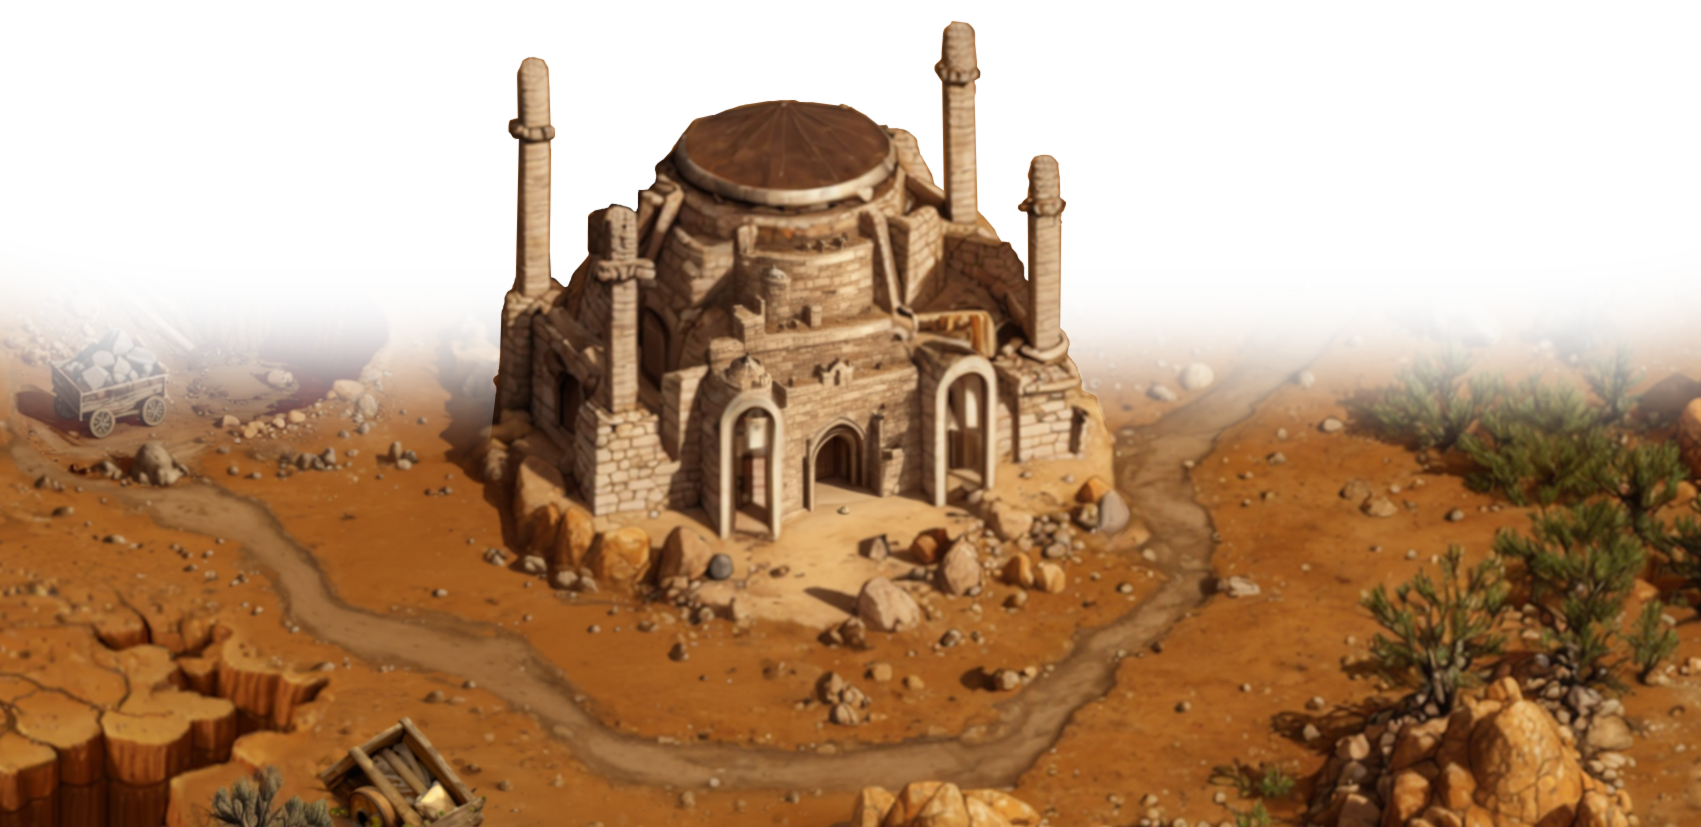
\includegraphics[width=1.01\paperwidth, keepaspectratio]{\art/castle_bottom.png}
    \thispagestyle{empty}
  };
\end{tikzpicture}}

\clearpage
In the heart of Jadame, the Factory rises as a beacon of progress amidst the desolation.
Born from the exodus of Halflings and refugees fleeing the Kreegan invasion of Eeofol, these innovators have forged a new future in Burton, igniting a wave of Factory towns across Terra Nova.

Here, mercenaries and artificers unite, commanding tamed exotic beasts and mechanical marvels in the Wasteland.
Armed with guns and flamethrowers, they stand ready to defend their realm.
The Factory buzzes with anticipation, eager for bold adventurers to step forth.

Will you embrace the challenge and harness the technological might of the Factory to etch your legend into the annals of history?

In this expansion for \textbf{Heroes of Might and Magic III: The Board Game}, you will discover a host of new features, including Quests, a new faction, a new scenario, a few optional rules for the Core Game, as well as a dedicated campaign.

\bigskip

\begin{multicols*}{2}
\tableofcontents
\vspace*{\fill}
\columnbreak
\vspace*{\fill}
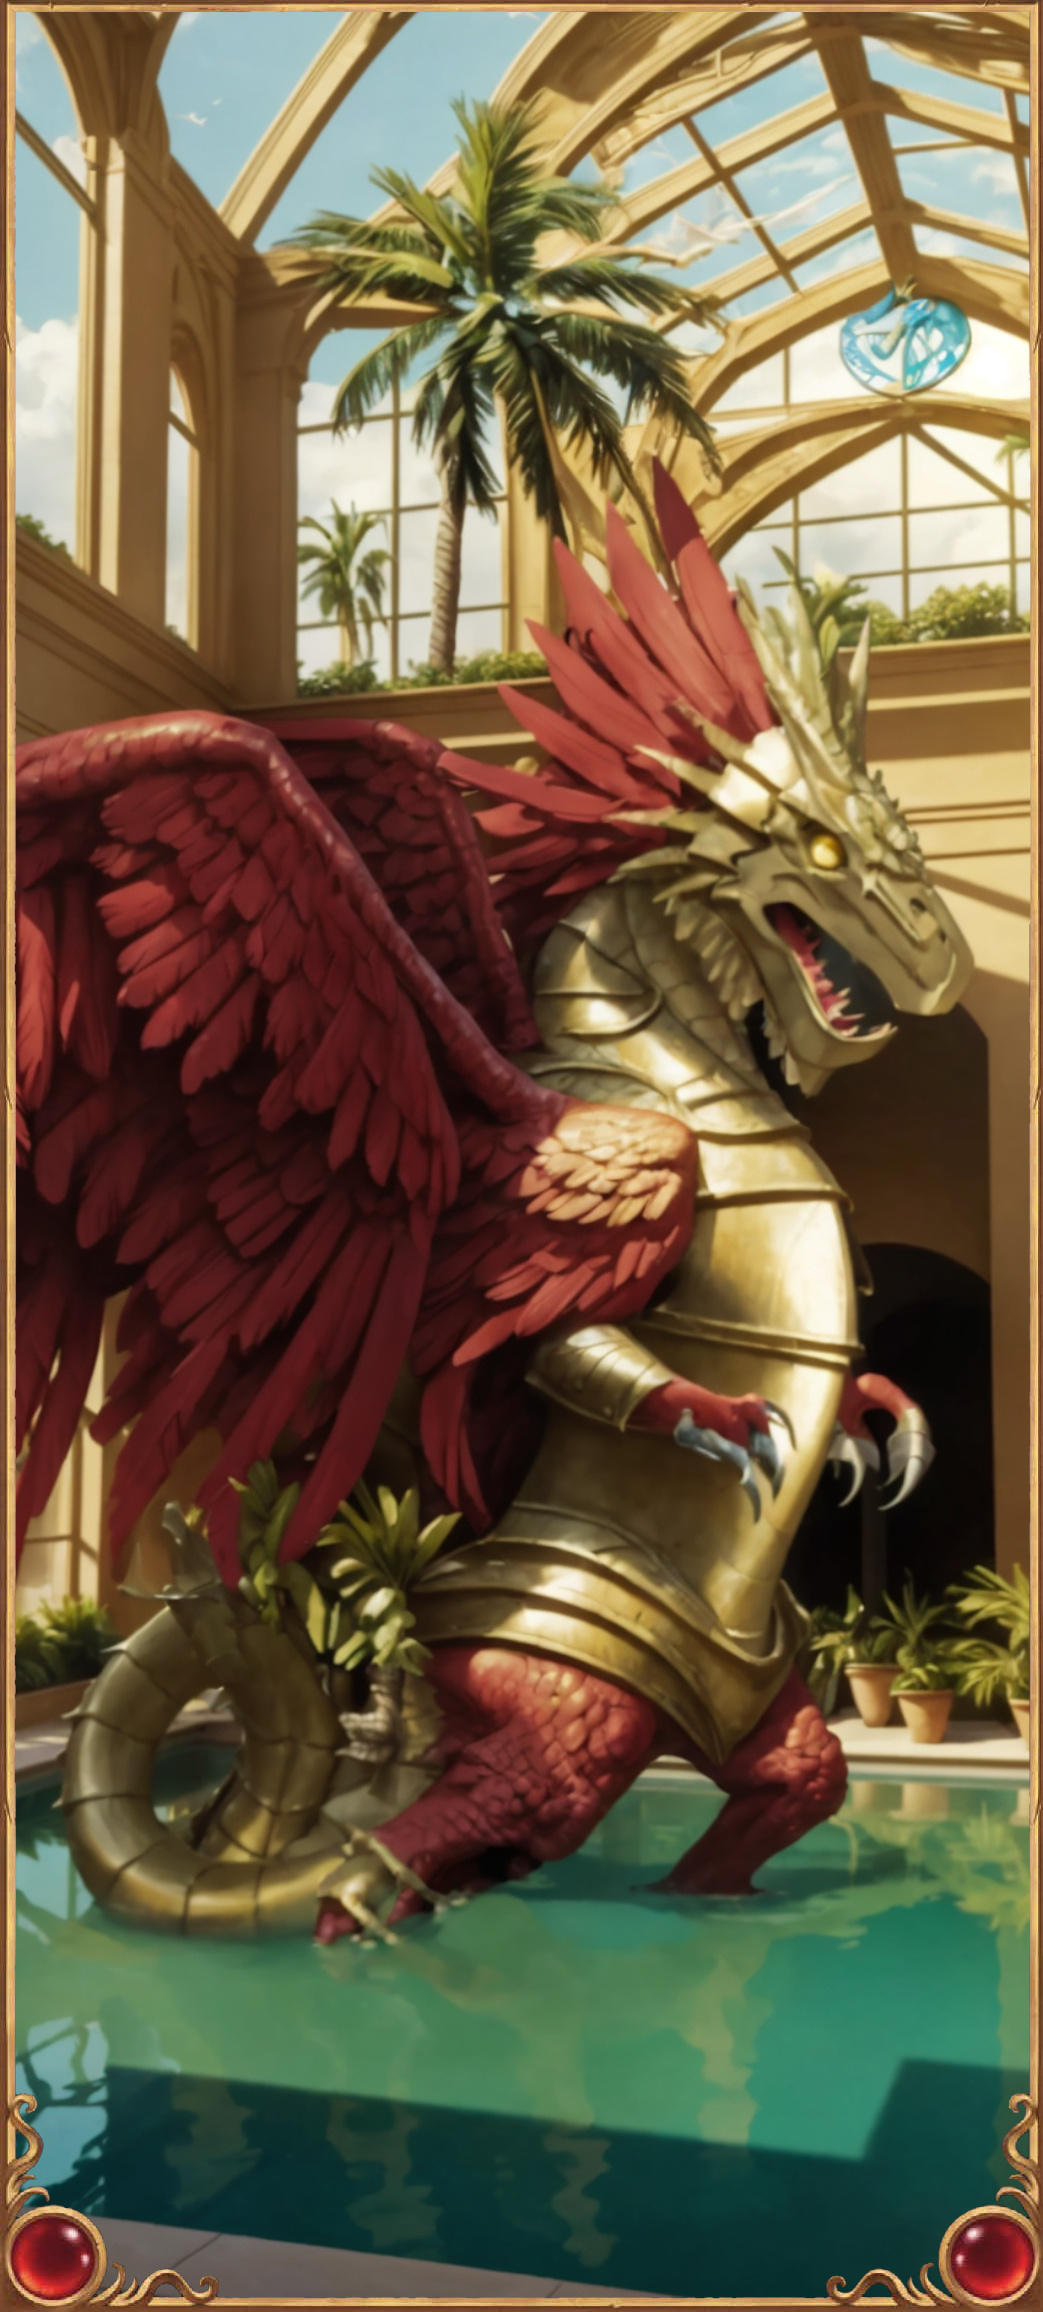
\includegraphics[width=\linewidth]{\art/crimson_couatl.jpg}
\end{multicols*}

\clearpage

% !TeX spellcheck = en_US
\addsection{Components}{\skills/luck.png}

\iftoggle{printable}{\vspace{-\baselineskip}}{}

This fan-made expansion is designed for self-printing and includes nearly all necessary components for gameplay.
However, certain elements, such as additional statistic cards, morale tokens, gold tokens, building material tokens, and valuable tokens, are not included.
Players using the Factory faction must source these components from other game expansions.

% TODO: Final number of components

\vspace*{1em}
\begin{multicols}{2}
  \textbf{Printable Components}\par
  \vspace{0.5em}
  \textbf{7 × Map Tiles:}
  \begin{itemize}
    \item 1 × Starting Tile
    \item 3 × Far Tiles
    \item 2 × Near Tiles
    \item 1 × Center Tile
  \end{itemize}
  \textbf{1 × Town Board}\par
  \textbf{1 × Mission Book}\par
  \textbf{3 × Hero Cards (double-sided)}\par
  \textbf{8 × Unit Cards}\par
  \textbf{7 × Town Building Tiles}\par
  \textbf{8 × Neutral Unit Cards}\par
  \textbf{18 × Specialty Cards}\par
  \textbf{? × Astrologers Proclaim Cards}\par
  \textbf{? × Spell Cards}\par
  \textbf{? × Ability Cards}\par
  \textbf{1 × Artifact Card}\par
  \textbf{4 × Mark Tokens}\par
  \textbf{1 × Build Token}\par
  \textbf{1 × Population Token}\par
  \textbf{1 × Spell Book Token}\par

\columnbreak
  \textbf{Necessary Replacements}\par
  \vspace{0.5em}
  \textbf{2 × Hero Miniatures}\par
  \textbf{8 × Unit Miniatures}\par
  \textbf{20 × Orange Acrylic Cubes}
  \bigskip

  \textbf{Borrow from Other Expansions:}\par
  \vspace{0.5em}
  Morale Token\par
  Building Material Tokens\par
  Valuable Tokens\par
  Gold Tokens\par
  Statistic Cards\par
  Black Acrylic Cubes\par
\end{multicols}


% !TeX spellcheck = en_US
\addsection{New Elements}{\skills/pathfinding.png}

\begin{multicols*}{2}

\begin{center}
  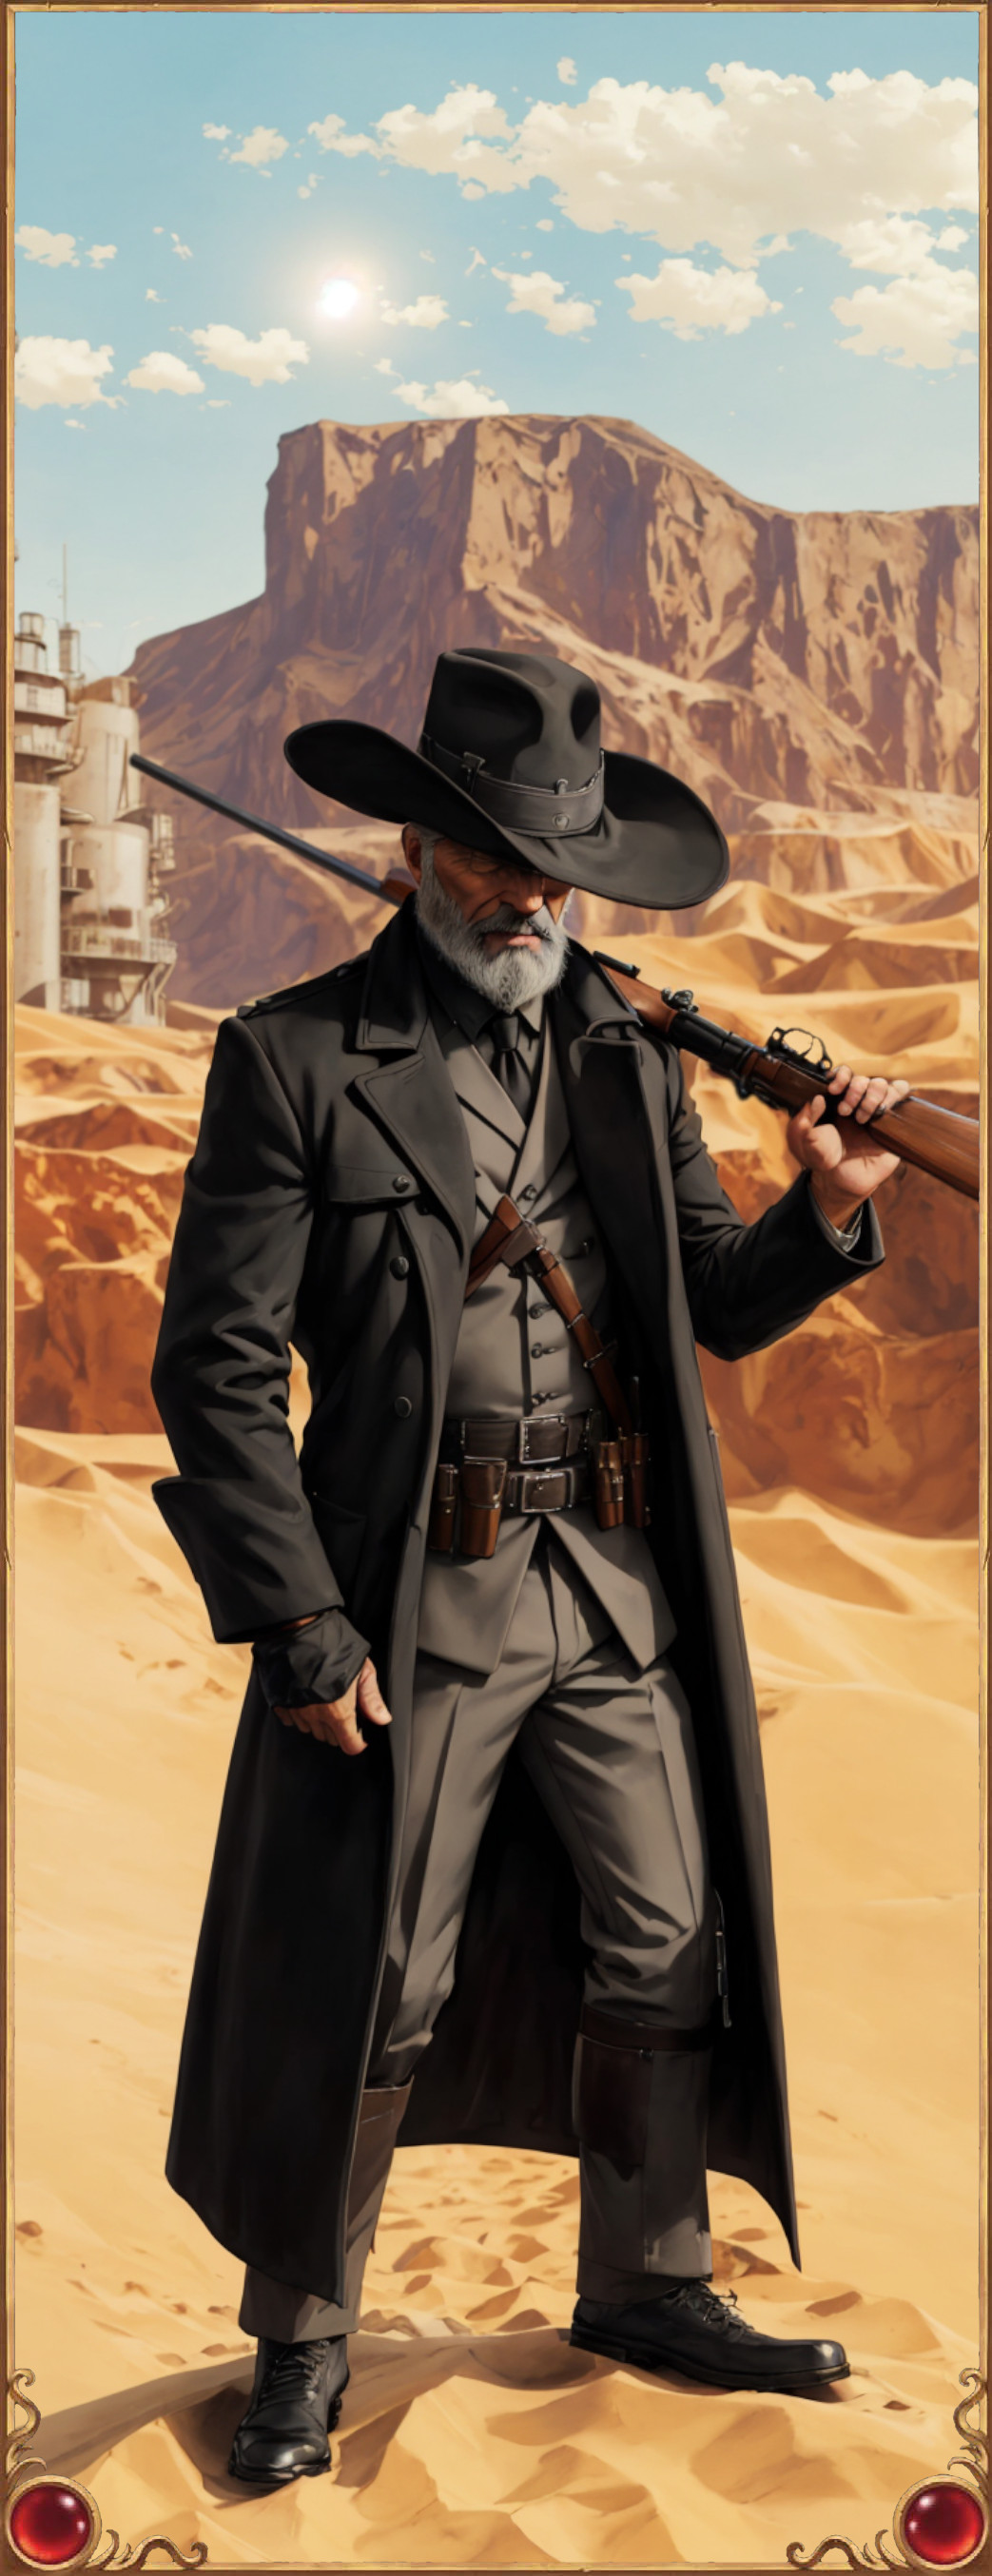
\includegraphics[width=\linewidth,height=\textheight,keepaspectratio]{\art/bounty_hunter.jpg}
\end{center}
\columnbreak

%\subsection*{\pagetarget{Quests}{Quests}}
\subheader{\pagetarget{Quests}{Quests}}

%Quests\index{Quests} are permanent Cards that can be bought at either a \pagelink{Trading Post}{Trading Post} or a \pagelink{War Machine Factory}{War Machine Factory}.
%If you buy one at the Trading Post, \textbf{you cannot use} any of the other normal functions of that Field during that Visit.
%War machines are also more expensive at the Trading Post.

The Factory expansion introduces “Quests\index{Quests} cards” \svg{quest_card}, which provide players with additional objectives to complete during the game.
Shuffle the Quest deck and place it face down near the game board.
Then, draw the top card and place it face up to create the discard pile.

{
  \bigskip
  \centering
  \begin{scriptsize}
    \begin{tikzpicture}
      \draw (0, 0) node[inner sep=0] {\makebox[\linewidth][c]{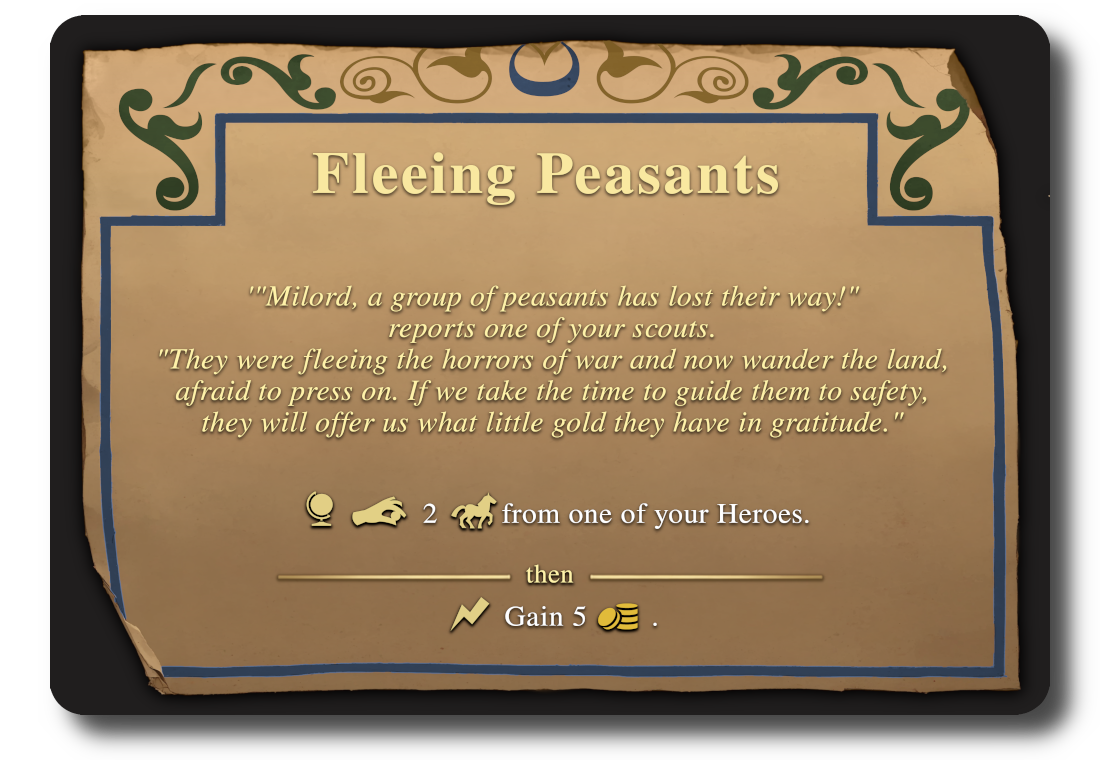
\includegraphics[width=\linewidth]{\cards/quest.png}}};
      \draw (0.4, 1.5) node {\encircle{\phantom{.}1\phantom{.}}};
      \draw (0, 0.2) node {\encircle{\phantom{.}2\phantom{.}}};
      \draw (-2.2, -0.95) node {\encircle{\phantom{.}3\phantom{.}}};
      \draw (-1.3, -1.7) node {\encircle{\phantom{.}4\phantom{.}}};
    \end{tikzpicture}
  \end{scriptsize}

  \footnotesize
  \textbf{\textit{\textcolor{darkcandyapplered}{Quest}}}

  \begin{multicols}{2}
    \begin{itemize}[itemsep=0pt, parsep=5pt, topsep=0pt, partopsep=0pt]
      \item[\textbf{1.}] Name
      \item[\textbf{2.}] Flavour text
      \item[\textbf{3.}] Requirement
      \item[\textbf{4.}] Reward
    \end{itemize}
  \end{multicols}
}

\subsection*{Structure of a Quest Card}

Each Quest card consists of two sections: Requirement and Reward.
There are two main types of Quests which differ significantly in the Requirement section:
\begin{itemize}
  \item \textbf{Non-Counter Quests} – These require a specific action to be performed (such as discarding cards or using abilities) or have a condition that must be met at a certain point in the game.
  The player may choose when to complete the Quest if the condition is met multiple times.
  \item \textbf{Counter Quests} – These require accumulating a certain number of \svg{quest_charge} tokens before they can be completed.
  When a player meets the condition to gain \svg{quest_charge}, they place a black cube on their Quest card.
  A Counter Quest can be completed at any time once it has at least the required number of \svg{quest_charge} tokens.
\end{itemize}

Once Quest is completed, the player immediately resolves the Reward effect and the card is removed from the game.

\subsection*{Acquiring and Managing Quests}
When a player gains a Quest, they place it face up next to their Hero or Town board.
A player may only have one active Quest at a time.
If a player gains a new Quest while already having an active one, they must discard the current Quest before accepting the new one.

Quests can be obtained from \pagelink{Seer’s Hut}{Seer’s Hut} locations, allowing a player to Search(2) Quests.
Seer’s Hut functions similarly to a Star Axis, meaning each player may use it only once.
Quests can also be acquired through new Astrologer effects and Event cards.
Just like other decks, Search(X) allows a player to take the top card from the discard pile.

By incorporating Quests into their strategy, players can gain powerful rewards that may turn the tide of the game.

{
  \bigskip
  \centering
  \begin{scriptsize}
    \begin{tikzpicture}
      \draw (0, 0) node[inner sep=0] {\makebox[0.47\linewidth][c]{
\includegraphics[width=0.47\linewidth]{\images/seers_hut.png}}};
    \end{tikzpicture}
  \end{scriptsize}

  \footnotesize
  \centering
  \textbf{\textit{\textcolor{darkcandyapplered}{Seer's Hut}}} \par
}

\vspace*{\fill}
\columnbreak


\subheader{\pagetarget{Map Locations}{Map Locations}}

In Factory Expansion, you will find more tiles with new locations to discover.
For the complete list of the locations, go to \pagelink{All Map Locations}{All Map Locations}.
% TODO: page link
\medskip

\subheader{\pagetarget{Mark Tokens}{Mark Tokens}}

\begin{tikzpicture}[overlay]
  \node at (7, 0) {
\includegraphics[width=0.2\linewidth]{\images/mark_token.png}};
\end{tikzpicture}\parbox{0.7\hsize}{Mark tokens are indicators placed on enemy units and are applied by units or abilities, enhancing strategic options during gameplay.}\par\smallskip
These tokens remain in play for the duration of the Combat and signify that the marked units are being targeted.
The specific effects of Mark tokens are detailed on the relevant cards, explaining how they influence the marked units.
Each unit can only have one Mark token applied to it.\par

\vfill
\hspace{2em}
\includegraphics[width=1.2\linewidth]{\art/implosion.png}
\vfill

\end{multicols*}


% !TeX spellcheck = en_US
\addsection{Map Locations}{\skills/logistics.png}

\begin{figure}[H]
  \begin{minipage}[t]{0.47\textwidth}
    \vspace{0pt}
    \centering
    \textbf{Town}\par
    \framedimage[\textwidth]{\map_locations/factory_town.jpg}
    \caption{\small Category: \textbf{Flaggable}\\
      This is a player’s starting field.
      If a player captures a Town, they gain a bonus depending on the scenario.}
  \end{minipage}\hfill
  \begin{minipage}[t]{0.47\textwidth}
    \vspace{0pt}
    \centering
    \captionsetup{singlelinecheck=off}
    \phantom{j}\textbf{Settlement}\par
    \framedimage[\textwidth]{\map_locations/factory_settlement.jpg}
    \caption{\small Category: \textbf{Flaggable}\\
      When you \textbf{Flag} a Settlement, you may select your reward from a number of bonuses.
      If you capture a Settlement that has not been previously owned by any player, you gain an extra bonus (see page 25, “Settlements” in the Core Rulebook).}
  \end{minipage}
\end{figure}

\begin{figure}[H]
  \begin{minipage}[t]{0.47\textwidth}
    \vspace{0pt}
    \centering
    \pagetarget{Derrick}{\textbf{Derrick}}\par
    \framedimage[\textwidth]{\map_locations/derrick.jpg}
    \caption{\small Category: \textbf{Visitable}\\
      Gain 3 \svg{gold}.
      For the purpose of timed events, treat Derrick as a Water Wheel.}
  \end{minipage}\hfill
  \begin{minipage}[t]{0.47\textwidth}
    \vspace{0pt}
    \centering
    \phantom{j}\textbf{Prospector}\par
    \framedimage[\textwidth]{\map_locations/prospector.jpg}
    \caption{\small Category: \textbf{Visitable}\\
      Gain 1 \svg{valuablegreater}.
      For the purpose of timed events, treat Prospector as a Windmill.}
  \end{minipage}
\end{figure}

\begin{figure}[H]
  \begin{minipage}[t]{0.47\textwidth}
    \vspace{0pt}
    \centering
    \textbf{Warlock's Lab}\par
    \framedimage[\linewidth]{\map_locations/warlocks_lab.jpg}
    \caption{\small Category: \textbf{Visitable}\\Remove 1 card from your hand to gain 1 \svg{valuablegreater}.}
  \end{minipage}\hfill
  \begin{minipage}[t]{0.47\textwidth}
    \vspace{0pt}
    \centering
    \phantom{j}\pagetarget{Grave}{\textbf{Grave}}\par
    \framedimage[\textwidth]{\map_locations/grave.jpg}
    \caption{\small Category: \textbf{Visitable}\\You may
      \svg{pay} 1 \svgeven{movement} to \textbf{Search(2)} \svg{artifact} and gain \svg{morale_negative}.
    }
  \end{minipage}
\end{figure}

\begin{figure}[H]
  \begin{minipage}[t]{0.47\textwidth}
    \vspace{0pt}
    \centering
    \phantom{j}\textbf{Watering Hole}\par
    \framedimage[\textwidth]{\map_locations/watering_hole.jpg}
    \caption{\small Category: \textbf{Revisitable}\\
      Immediately end your turn upon landing on this tile, next turn gain 1 \svgeven{movement}.
      It lasts for only one Turn.
    }
  \end{minipage}\hfill
  \begin{minipage}[t]{0.47\textwidth}
    \vspace{0pt}
    \centering
    \pagetarget{Trailblazer}{\textbf{Trailblazer}}\par
    \framedimage[\textwidth]{\map_locations/trailblazer.jpg}
    \caption{\small Category: \textbf{Revisitable}\\
      Gain 1 \svgeven{movement}.
      It lasts for only one Turn.
    }
  \end{minipage}
\end{figure}

\begin{figure}[H]
  \begin{minipage}[t]{0.47\textwidth}
    \vspace{0pt}
    \centering
    \textbf{Airship Yard}\par
    \framedimage[\linewidth]{\map_locations/airship_yard.jpg}
    \caption{\small Category: \textbf{Revisitable}\\You may
      \svg{pay_v2} 3 \svg{gold} to gain 2 \svgeven{movement}.
    During this turn, your Hero can move through blocked fields (but cannot end their movement there).}
  \end{minipage}\hfill
\end{figure}



%\clearpage
%\phantomsection
%\addcontentsline{toc}{section}{Scenarios}
%% !TeX spellcheck = en_US
\addscenariosection{1}{Cooperative Scenario}{...}{\images/title.png}

\begin{multicols*}{2}

\textit{... 1--2 two paragraphs to set the story ...}

\subsection*{\MakeUppercase{Scenario Length}}

This Scenario is played over ... Rounds.

\subsection*{\MakeUppercase{Player Setup}}

\textbf{Player Count:} ...

\textbf{Starting Resources:} X \svg{gold}, Y \svg{building_materials}, Z \svg{valuables}

\textbf{Starting Income:} A \svg{gold}, B \svg{building_materials}, C \svg{valuables}

\textbf{Starting Units:}
\begin{itemize}
  \item A Few \svgunit{bronze}...
  \item A Pack \svgunit{silver}...
  \item \svgunit{golden}
  \item \svgunit{azure}
\end{itemize}

\textbf{Town Buildings:} \svgunit{bronze} Dwelling...

\textbf{Map Tile Pool:} Each player takes X [random] Near/Far Map (A--B) Tiles...

\textbf{Additional Bonus:} Choose one of the following options:

\begin{itemize}
    \item ...
\end{itemize}

\subsection*{\MakeUppercase{Map Setup}}

Take the following Map Tiles and arrange them as shown in the Scenario map layout:
\begin{itemize}
  \item W × Starting (I) Map Tile
  \item X × Far (II--III) Map Tile
  \item Y × Near (IV--V) Map Tile
  \item Z × Center (VI--VII) Map Tile
\end{itemize}

\subsection*{\MakeUppercase{Victory Conditions}}
...

\subsection*{\MakeUppercase{Defeat Conditions}}
...

\subsection*{\MakeUppercase{Timed Events}}

\textbf{\nth{2} Round:}
\begin{itemize}
  \item ...
  \item ...
\end{itemize}

% IF THERE ARE OVERLAPPING EVENTS, FOLLOW BELOW STRUCTURE, IN CHRONOLOGICAL ORDER
%
% \textbf{\nth{7} and \nth{8} Rounds:}
% \begin{itemize}
%   \item ...
% \end{itemize}
%
% \textbf{\nth{9} Round:}
% \begin{itemize}
%   \item Repeat Timed Events of Round 6.
% \end{itemize}
%
% \textbf{\nth{10} Round:}
% \begin{itemize}
%   \item Repeat Timed Events of Rounds 7 and 8.
% \end{itemize}

\subsection*{\MakeUppercase{Additional Rules}}

\begin{itemize}
    \item ...
\end{itemize}

\end{multicols*}

% Uncomment if you need a table to define Unit strengths or other parameters of the game
% \hommtable[]{12}{
%   \centering
%   \medskip
%   \textbf{... title ...}\\
%   \bigskip

%   \newcommand{\bronze}[0]{\svg[12]{bronze}}
%   \newcommand{\silver}[0]{\svg[12]{silver}}
%   \newcommand{\golden}[0]{\svg[12]{golden}}
%   \newcommand{\azure}[0]{\svg[12]{azure}}

%   \begin{tabularx}{\linewidth}{p{0.15\linewidth}XXXX} & \darkcell{Column 1 name} & \darkcell{Column 2 name}\\
%     \darkcell[1.4]{Row 1 name}
%         & \lightcell[1.4]{\bronze \silver \golden \azure}
%         & \lightcell[1.4]{... other stuff ...} \\
%         \darkcell[1.4]{Row 1 name}
%         & \lightcell[1.4]{\bronze \silver \golden \azure}
%         & \lightcell[1.4]{... other stuff ...} \\
%   \end{tabularx}
% }

% Uncomment and link a map image
% \vspace{3em}
% \begin{center}
%   \includegraphics[width=0.6\paperwidth]{\_assets/maps/your_map.png}
% \end{center}


%\clearpage
%\phantomsection
%\addcontentsline{toc}{subsection}{Factory Campaign}

%\sectionheadertext{Factory Campaign}
%\section{Factory Campaign}

% !TeX spellcheck = en_US
\cleardoublepage\phantomsection\addcontentsline{toc}{section}{\protect\numberline{}\mbox{Factory Campaign}}
\addscenariosection[subsection]{1}{Factory Campaign-Forged in Fire}{1. World on Fire}{\spells/meteor_shower.png}

\begin{multicols*}{2}

\subsection*{\MakeUppercase{Scenario Length}}

This Scenario plays out over ... Rounds.

\subsection*{\MakeUppercase{Player Setup}}

\textbf{Faction:} Factory

\textbf{Faction Hero:} Henrietta

\textbf{Starting Resources:} X \svg{gold}, Y \svg{building_materials}, Z \svg{valuables}

\textbf{Starting Income:} A \svg{gold}, B \svg{building_materials}, C \svg{valuables}

\textbf{Starting Units:}
\begin{itemize}
  \item A Few \svgunit{bronze}...
  \item A Pack \svgunit{silver}...
  \item \svgunit{golden}
  \item \svg{azure}
\end{itemize}

\textbf{Town Buildings:} \svgunit{bronze} Dwelling...

\textbf{Bonus:} Choose one of the following options:
\begin{itemize}
    \item ...
\end{itemize}

\subsection*{\MakeUppercase{AI Hero Setup}}

\textbf{Faction:} ...

\textbf{Enemy Army:} ...

\textbf{Enemy Deck:} ...

\textbf{Enemy Spell Deck:} ...

\textbf{Enemy Skills:} ...

\textbf{Special:} ...

\subsection*{\MakeUppercase{Map Setup}}

Take the following Map Tiles and arrange them as shown in the Scenario map layout:

\textbf{X × Starting (I) Map Tile}
\begin{itemize}
    \item ... additional constraints ...
\end{itemize}

\textbf{Y × Far (II--III) Map Tile}

\textbf{Z × Near (IV--V) Map Tile}

\subsection*{\MakeUppercase{Heroes Placement}}

... describe how your and enemy Heroes will be placed ...

\subsection*{\MakeUppercase{Victory Conditions}}
...

\subsection*{\MakeUppercase{Defeat Conditions}}
...

\subsection*{\MakeUppercase{Timed Events}}

% Unless you have a rich and non-linear story, write it under specific
% Rounds here.
%
% Otherwise create a new subsection "The Story" at the end and refer to it.

\textbf{\nth{2} Round:}
\begin{itemize}
  \item ...
  \item ...
\end{itemize}

% IF THERE ARE OVERLAPPING EVENTS, FOLLOW BELOW STRUCTURE, IN CHRONOLOGICAL ORDER
%
% \textbf{\nth{7} and \nth{8} Rounds:}
% \begin{itemize}
%   \item ...
% \end{itemize}
%
% \textbf{\nth{9} Round:}
% \begin{itemize}
%   \item Repeat Timed Events of Round 6.
% \end{itemize}
%
% \textbf{\nth{10} Round:}
% \begin{itemize}
%   \item Repeat Timed Events of Rounds 7 and 8.
% \end{itemize}

\subsection*{\MakeUppercase{Additional Rules}}

During this ``... Faction ...'' Campaign Scenario, the following rules apply:

\begin{itemize}
  \item ...
\end{itemize}

\end{multicols*}

\newpage

% NOTE: The last page of Scenario preparation should use
% multicols instead of multicols* to create space for map.
% \begin{multicols}{2}
% ... your content that overflows to the second page ...
% \end{multicols}

% Uncomment and link a map image
% \vspace{3em}
% \begin{center}
%   \includegraphics[width=0.6\paperwidth]{\_assets/maps/sentinels.png}
% \end{center}

\newpage

\begin{multicols*}{2}

\subsection*{\MakeUppercase{The Story}}

... put your immersive story here ...

\end{multicols*}


% !TeX spellcheck = en_US

\addscenariosection[subsection]{1}{Factory Campaign-Forged in Fire}{2. Beyond the Horizon}{\skills/scouting.png}

\begin{multicols*}{2}

\subsection*{\MakeUppercase{Scenario Length}}

This Scenario plays out over ... Rounds.

\subsection*{\MakeUppercase{Player Setup}}

\textbf{Faction:} Factory

\textbf{Faction Hero:} Henrietta

\textbf{Starting Resources:} X \svg{gold}, Y \svg{building_materials}, Z \svg{valuables}

\textbf{Starting Income:} A \svg{gold}, B \svg{building_materials}, C \svg{valuables}

\textbf{Starting Units:}
\begin{itemize}
  \item A Few \svgunit{bronze}...
  \item A Pack \svgunit{silver}...
  \item \svgunit{golden}
  \item \svg{azure}
\end{itemize}

\textbf{Town Buildings:} \svgunit{bronze} Dwelling...

\textbf{Bonus:} Choose one of the following options:
\begin{itemize}
    \item ...
\end{itemize}

\subsection*{\MakeUppercase{AI Hero Setup}}

\textbf{Faction:} ...

\textbf{Enemy Army:} ...

\textbf{Enemy Deck:} ...

\textbf{Enemy Spell Deck:} ...

\textbf{Enemy Skills:} ...

\textbf{Special:} ...

\subsection*{\MakeUppercase{Map Setup}}

Take the following Map Tiles and arrange them as shown in the Scenario map layout:

\textbf{X × Starting (I) Map Tile}
\begin{itemize}
    \item ... additional constraints ...
\end{itemize}

\textbf{Y × Far (II--III) Map Tile}

\textbf{Z × Near (IV--V) Map Tile}

\subsection*{\MakeUppercase{Heroes Placement}}

... describe how your and enemy Heroes will be placed ...

\subsection*{\MakeUppercase{Victory Conditions}}
...

\subsection*{\MakeUppercase{Defeat Conditions}}
...

\subsection*{\MakeUppercase{Timed Events}}

% Unless you have a rich and non-linear story, write it under specific
% Rounds here.
%
% Otherwise create a new subsection "The Story" at the end and refer to it.

\textbf{\nth{2} Round:}
\begin{itemize}
  \item ...
  \item ...
\end{itemize}

% IF THERE ARE OVERLAPPING EVENTS, FOLLOW BELOW STRUCTURE, IN CHRONOLOGICAL ORDER
%
% \textbf{\nth{7} and \nth{8} Rounds:}
% \begin{itemize}
%   \item ...
% \end{itemize}
%
% \textbf{\nth{9} Round:}
% \begin{itemize}
%   \item Repeat Timed Events of Round 6.
% \end{itemize}
%
% \textbf{\nth{10} Round:}
% \begin{itemize}
%   \item Repeat Timed Events of Rounds 7 and 8.
% \end{itemize}

\subsection*{\MakeUppercase{Additional Rules}}

During this ``... Faction ...'' Campaign Scenario, the following rules apply:

\begin{itemize}
  \item ...
\end{itemize}

\end{multicols*}

\newpage

% NOTE: The last page of Scenario preparation should use
% multicols instead of multicols* to create space for map.
% \begin{multicols}{2}
% ... your content that overflows to the second page ...
% \end{multicols}

% Uncomment and link a map image
% \vspace{3em}
% \begin{center}
%   \includegraphics[width=0.6\paperwidth]{\_assets/maps/sentinels.png}
% \end{center}

\newpage

\begin{multicols*}{2}

\subsection*{\MakeUppercase{The Story}}

... put your immersive story here ...

\end{multicols*}


\iftoggle{printable_notes_page}{\include{\sections/notes.tex}}{}

% !TeX spellcheck = en_US

\addsection{Credits}{\images/experience.png}

\iftoggle{printable}{\vspace{-\baselineskip}}{}

\bigbreak

\begin{multicols*}{2}

  % TODO: List all contributors

\textbf{Author}: Piotr Bruzda

\textbf{Expansion Design}: Re4XN

\textbf{Graphics Editing}: Piotr Bruzda, Fomx

\textbf{Playtesting \& Balancing}: TODO: To be completed

\textbf{Tabletop Simulator Addon}: invoceusse

\textbf{Proofreading}: TODO: To be completed

\textbf{Spellchecking}: TODO: To be completed

\textbf{GitHub Engineering \& Mission Book Layout (based on work from the \href{\originalrepourl}{Rulebook Rewrite project})}: Hermanni Karppela, Andrzej Wiącek, Alexey Sokolov, Vadász András, Rickard Nilsson, Joris de Kleer, Kate Katrankova

\textbf{Special Thanks}: HotA Crew for their exceptional work in creating the Factory in the Horn of the Abyss expansion, which serves as the foundation for this adaptation.
Everyone from Archon Studio for producing the game and answering our incessant queries about rules and other topics.
Jon Van Caneghem and everyone involved with the development of the original video game.
Everyone who has supported the project with suggestions, corrections, image resources, and words of encouragement either on Discord or BoardGameGeek.

\textbf{Artwork Borrowed from Official Release was Made by}: Tomasz Badalski, Yoann Boissonnet, Shen Fei, Viviane Tybusch Souza, Iana Vengerova, Bartosz Winkler

\columnbreak

\vspace*{\fill}

\includegraphics[width=1.3\linewidth]{\art/genie.png}

\vspace*{\fill}

\end{multicols*}


\iftoggle{printable}{\include{\sections/index.tex}}{}

% !TeX spellcheck = en_US

\restoregeometry

\pagestyle{empty}
\iftoggle{noartbackground}{}{
  \begin{tikzpicture}[remember picture, overlay, inner sep=10pt]
    \node(cover)[anchor=center] at (current page.center) {
      
\includegraphics[height=\paperheight, keepaspectratio]{\layout/back.jpg}
    };
  \end{tikzpicture}
}


\end{document}
